En este capítulo, primero se justifica la elección de los datasets empleados durante los experimentos propuestos para responder a las preguntas de investigación. Después, se describe el diseño de dichos experimentos. Finalmente, se ofrecen algunos detalles técnicos de la implementación, así como las métricas recogidas durante la fase de ejecución.

%%%%%%%%%%%%%%%%%%%%%%%%%%%%%%%%%%%%%%%%%%%%%%%%%%%%%%%%%%%%%%
\section{Justificación de los datasets\label{SEC:DATASETS}}
%%%%%%%%%%%%%%%%%%%%%%%%%%%%%%%%%%%%%%%%%%%%%%%%%%%%%%%%%%%%%%

Como ya se ha mencionado en la Sección \ref{SEC:RESGAPS}, la pregunta \textbf{RQ2} (sobre la necesidad de conocer de antemano el desbalanceo del dataset) requiere un estudio sobre un dataset bajo diferentes grados de desbalanceo, de forma que se pretende observar las variaciones entre escenarios. Por otra parte, la resolución de la \textbf{RQ3} (sobre cómo afecta la complejidad del dataset al método a elegir) pasa por realizar los experimentos sobre dos conjuntos de datos con distinta complejidad.
El primero, y más acorde al dominio de este trabajo, se compone de imágenes faciales de hombres y mujeres, sobre las que se han probado dos escenarios de desbalanceo distintos. Se trata del dataset ``complejo'', y sobre él se van a crear varios escenarios de desbalanceo. El segundo consiste en un conjunto de imágenes con una gran similitud entre muestras, por lo que constituye el dataset ``sencillo''.

En primer lugar, para el dominio del reconocimiento de género facial, de entre los tres datasets más mencionados en la bibliografía (FERET, UTKFace e IMDB-WIKI \cite{yilmaz2021evolutionary,loo2018influence,islam2020human,garain2021gra_net,agbo2020deeply,dwivedi2019review,agbo2019face,khryashchev2013adaptive,tianyu2018human,vallimeena2019cnn}), dos presentan ciertos inconvenientes que motivan descartarlos:

\begin{enumerate}
    \fontsize{11pt}{12pt}\selectfont
    \item \textbf{FERET}\footnote{Fuente: https://www.nist.gov/itl/products-and-services/color-feret-database} \cite{yilmaz2021evolutionary,loo2018influence,dwivedi2019review,khryashchev2013adaptive,tianyu2018human,vallimeena2019cnn}: no está disponible al dominio público. % y es difícil de manejar.
    \item \textbf{IMDB-WIKI}\footnote{Fuente: https://data.vision.ee.ethz.ch/cvl/rrothe/imdb-wiki/} \cite{islam2020human,agbo2020deeply,agbo2019face}: pese a contener información de género y raza para muchos miles de instancias, exige que se trate con \textsc{Matlab}, lo cual dificulta su integración en el ecosistema de PyTorch utilizado. 
\end{enumerate}

Es por ello que se elige el dataset UTKFace \cite{UTKFACE,zhifei2017cvpr}, que dispone de tres clases: género, edad y raza para 23.708 imágenes faciales a color, y en diversos escenarios de postura, resolución e iluminación. Esta variedad asegura que el modelo pueda aprender las características diferenciadoras de hombres y mujeres en cuantos más escenarios de etnia, edad y condiciones posible. Su distribución de género, ilustrada en la Figura \ref{FIG:UTKFace_study}, es bastante igualitaria, con lo que permite generar artificialmente diferentes escenarios de desbalanceo. %Su distribución de clases se ejemplifica en la Figura \ref{FIG:UTKFace_study}.

\begin{figure}[Estudio UTKFace]{FIG:UTKFace_study}{Estudio estadístico del dataset UTKFace.}
    \centering
    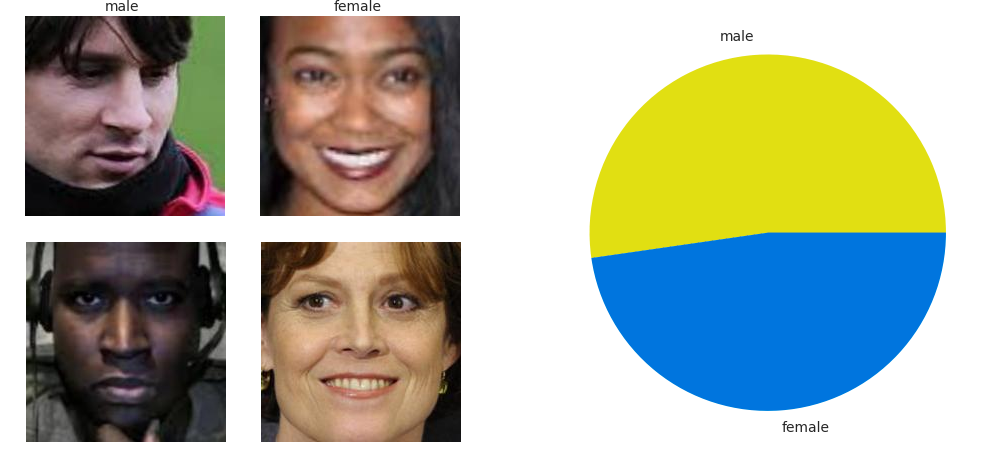
\includegraphics[width=14cm]{img/utk_gender.png}
\end{figure}

En segundo lugar, se realizan los experimentos sobre un conjunto de datos con una gran similitud entre muestras, menos ``complejo''. En concreto, se ha escogido el dataset PlantVillage \cite{hughes2015open}, por varios motivos. Primero, sus muestras recogen imágenes de plantas de tomate ``sanas'' e ``infectadas'', tomadas sobre el mismo fondo e iluminación. Esta alta similaridad entre muestras hace que PlantVillage sea más simple que UTKFace. El otro motivo de escoger este dataset es que se emplea en la revisión de \citet{nafi2020addressing}, en la que se demuestra empíricamente la idoneidad de las WGAN sobre otras técnicas a nivel de datos, pudiendo encontrar así un punto común sobre el que experimentar. Como este trabajo se centra en los problemas de clasificación binaria, se utiliza un subconjunto de este dataset. En concreto, solo se preservan las clases para tomates sanos, y para tomates infectados con el ``\textit{mosaic virus}'', pues es el escenario de referencia descrito en \citet{nafi2020addressing} (Figura \ref{FIG:plantvillage_study}). Así, el subconjunto de PlantVillage usado consta de 1964 imágenes: 1591 para tomates sanos, y 373 para los infectados (es decir, existe un desbalanceo por defecto).

\begin{figure}[Estudio PlantVillage]{FIG:plantvillage_study}{Estudio estadístico del dataset PlantVillage.}
    \centering
    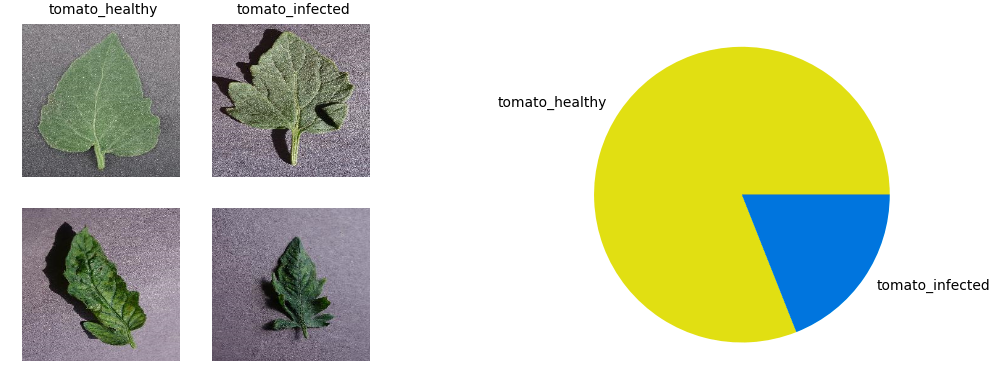
\includegraphics[width=12cm]{img/plantvillage_dist.png}
\end{figure}

En resumen, a partir de los dos datasets expuestos, se han creado los siguientes escenarios en los experimentos. Junto al alias de cada dataset se indica su IR (Ecuación \ref{EQ:IMBRAT}):

\begin{enumerate}
    \fontsize{11pt}{12pt}\selectfont
    \item \textbf{UTKFaceBias} [IR = 4,23 (12391 hombres, 3056 mujeres)]: imágenes faciales de hombres y mujeres con un escenario de balanceo 4 a 1, en desventaja para los hombres (proveniente del dataset UTKFace \cite{UTKFACE,zhifei2017cvpr}).
    \item \textbf{UTKFaceFull} [IR = 1,095 (12391 hombres, 11317 mujeres)]: imágenes faciales de hombres y mujeres con clases balanceadas (mismo dataset que \textbf{UTKFaceBias}). Al incluir dos escenarios de balanceo para el mismo dataset, se pretende responder a la \textbf{RQ2}.
    \item \textbf{PlantVillage} [IR = 4,23 (1591	tomates sanos, 373 infectados)]: imágenes de plantas de tomates sanos e infectados con un escenario de balanceo 4 a 1, en desventaja para los infectados (proveniente del dataset PlantVillage \cite{hughes2015open}). Esto nos permite experimentar sobre distintos escenarios de complejidad y dar respuesta a la \textbf{RQ3}.
\end{enumerate}

Como puede observarse, el desbalanceo de \textbf{UTKFaceBias} y \textbf{PlantVillage} es el mismo: 4,23 (que es el IR ``nativo'' de PlantVillage). \textbf{UTKFaceBias} se ha adaptado a este IR para que las comparativas entre datasets con desbalanceo estén en la mayor igualdad de condiciones.



%%%%%%%%%%%%%%%%%%%%%%%%%%%%%%%%%%%%%%%%%%%%%%%%%%%%%%%%%%%%%%
\section{Diseño de los experimentos\label{SEC:EXPERIMENTOS}}
%%%%%%%%%%%%%%%%%%%%%%%%%%%%%%%%%%%%%%%%%%%%%%%%%%%%%%%%%%%%%%

En relación con la \textbf{RQ1} (sobre cuál de las dos familias de técnicas mitigantes del desbalanceo es más adecuada), para cada uno de los tres datasets enumerados, se entrenan los modelos del \textsc{Capítulo \ref{CAP:METODO}}. Poniendo en común los conjuntos de datos y el objetivo de cada experimento, se pretende que las métricas de rendimiento recogidas sean coherentes y significativas para obtener resultados concluyentes. Los modelos lanzados sobre cada uno de los tres datasets son los siguientes:

\begin{enumerate}
    \fontsize{11pt}{12pt}\selectfont
    \item \textbf{Baseline}: se entrena un modelo de clasificación estándar sobre los datos. Se utiliza como función de pérdida la de entropía cruzada (\textit{Cross Entropy Loss}). Esta es la referencia contra la que se mide la mejora (o ausencia de mejora) de los métodos de mitigación del desbalanceo seleccionados, y de la Loss Focal Difusa.
    \item \textbf{WGAN}: consiste en el mismo modelo y configuración que \textbf{Baseline}, pero en este caso el desbalanceo de cada dataset se compensa por medio de la generación sintética de muestras con una WGAN entrenada previamente sobre la clase minoritaria. El código es el presentado en \citet{arjovsky2017wasserstein}.
    \item \textbf{Loss Focal}: al modelo de referencia del \textbf{Baseline} se le cambia la función de pérdida por una implementación oficial de la Loss Focal (código provisto en \citet{lin2017focal}), probando distintos valores de $\gamma$.
    \item \textbf{Loss Focal Difusa}: se trata de casi el mismo experimento que \textbf{Loss Focal}, pero incluyendo la actualización dinámica del hiperparámetro $\gamma$ de la función de pérdida por medio del Sistema de Control Difuso diseñado en este proyecto.
    \item \textbf{PRM-IM}: aplica el sistema de \citet{liu2022solving} de repetición de la clase minoritaria junto a subconjuntos de la mayoritaria, unido a un extractor de características formado por dos CNNs (\textit{Xception} \cite{chollet2017xception}, y \textit{ResNet50} \cite{he2016deep}) y una capa densamente conexa común. Se usa la entropía cruzada como función de pérdida.
    \item \textbf{CoSenCNN}: replica el escenario descrito en \citet{khan2017cost} para la red sensible a costes, utilizando como clasificador la misma arqutiectura de CNN que \textbf{Baseline}. La implementación es la propuesta en \citet{khan2017cost}.
\end{enumerate}






%%%%%%%%%%%%%%%%%%%%%%%%%%%%%%%%%%%%%%%%%%%%%%%%%%%%%%%%%%%%%%
\section{Detalles de implementación\label{SEC:IMPLEMENTACION}}
%%%%%%%%%%%%%%%%%%%%%%%%%%%%%%%%%%%%%%%%%%%%%%%%%%%%%%%%%%%%%%

% En esta sección se describen algunos detalles técnicos de la implementación.
Los experimentos y modelos han sido escritos en el lenguaje de programación Python, haciendo uso de las librerías de aprendizaje automático PyTorch \cite{NEURIPS2019_9015}, TensorFlow \cite{tensorflow2015-whitepaper}, Scikit-Learn \cite{scikit-learn} y FuzzyLogic \cite{Kiefner_FuzzyLogic_for_Python_2022}. Tanto para la \textbf{WGAN} \cite{arjovsky2017wasserstein}, como para la \textbf{CoSenCNN} \cite{khan2017cost}, se utilizan las implementaciones originales, adaptándolas al entorno de PyTorch. A nivel hardware, se dispone de una tarjeta gráfica NVIDIA GeForce GTX 1070, sistema operativo Windows 11 y CPU Intel Core i7-8700K de 3.70GHz .

En cuanto al clasificador de los experimentos \textbf{Baseline}, \textbf{WGAN}, \textbf{Loss Focal} y \textbf{Loss Focal Difusa}, la bibliografía estudiada motiva que sea una CNN \cite{wu2020gender,islam2020human,garain2021gra_net,agbo2020deeply,sumi2021human,zhang2020gender}. En este punto, hay dos opciones: bien diseñar la red desde cero, o bien aprovechar alguna arquitectura existente en el estado del arte. Se opta por la segunda opción, debido a que en los últimos años los modelos disponibles son bastante difíciles de superar, y el margen de aportación es limitado para la naturaleza de este trabajo. El modelo elegido es la arquitectura ResNet \cite{he2016deep}, concretamente ResNet-50, y al igual que otros estudios, se usa la técnica de \textit{transfer learning} para adaptarlo a nuestras necesidades particulares. Se trata de un modelo entrenado en el dataset ImageNet, compuesto de cientos de miles de imágenes pertenecientes a 1000 categorías. En el \textit{Reto de Reconocimiento Visual a Gran Escala} \cite{ILSVRC}, ResNet es una de las arquitecturas con mejores resultados.

% \begin{figure}[Clasificación de ILSVRC]{FIG:ILSVRC_comparison}{Clasificación de ResNet en el reto ILSVRC.}
%     \centering
%     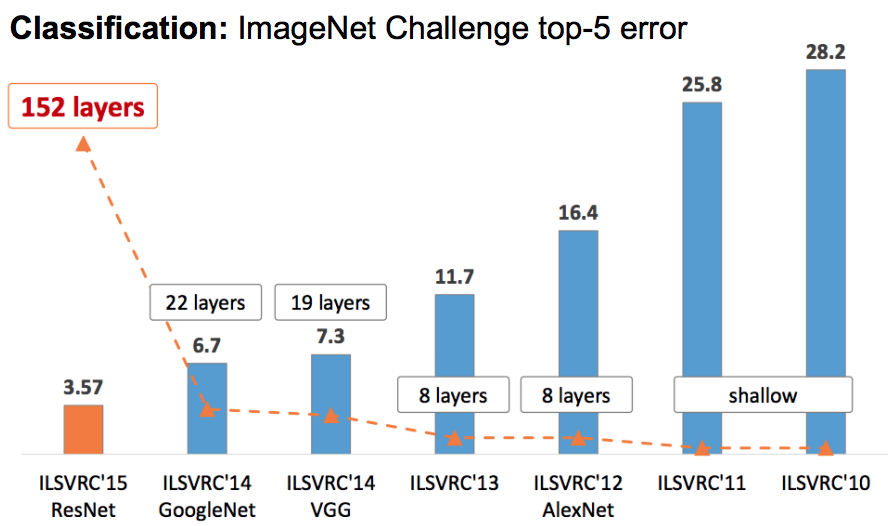
\includegraphics[width=10cm]{img/ILSVRC_comparison.png}
% \end{figure}

Exceptuando los experimentos de la \textbf{Loss Focal}, la \textbf{Loss Focal Difusa} y la \textbf{CoSen CNN}, el resto de clasificadores (\textbf{Baseline}, \textbf{WGAN} y \textbf{PRM-IM}) utilizan la función de pérdida por entropía cruzada, por ser la más usada en la bibliografía \cite{wu2020gender,islam2020human,garain2021gra_net,agbo2020deeply,sumi2021human,zhang2020gender}. Otros aspectos que cabe subrayar son el uso de planificadores de la tasa de aprendizaje (del inglés \textit{learning rate schedulers}) y el optimizador elegido, cuando estos no vienen especificados por la implementación original. En ambos casos se han seguido las recomendaciones de la bibliografía \cite{wu2020gender,islam2020human,garain2021gra_net,agbo2020deeply,sumi2021human,zhang2020gender}: las redes utilizan un planificador ``\textit{One-Cycle}'' con tasa máxima de 0.01; y un optimizador Adam, el cual suele ser preferido frente a otros como el de SGD por la mayoría de autores.

Para encontrar la configuración óptima de cada experimento, cada bucle de entrenamiento-validación se ha lanzado con diferentes combinaciones de hiperparámtros en lo que se conoce como búsqueda en malla (\textit{grid search}) con validación cruzada de 3 iteraciones. Por último, cada uno de los bucles de entrenamiento-validación realiza una validación cruzada de 5 iteraciones (exceptuando \textbf{PRM-IM}, cuyo algoritmo de entrenamiento es el de la Sección \ref{SUBSEC:PRMIM}). La Tabla \ref{TB:RESUMEN_HIPERPARAMS} resume los distintos hiperparámetros optimizados en el conjunto de los experimentos:

\begin{table}[Resumen de hiperparámetros]{TB:RESUMEN_HIPERPARAMS}{Hiperparámetros optimizados a lo largo de los distintos experimentos.}
    \small
    \begin{tabular}{|l|p{13cm}|}
        \hline
        \textsc{Hiperparámetro} & \textsc{Descripción} \\
        \hline
        \texttt{epochs} & Número de iteraciones dentro de uno de los 5 bucles de entrenamiento-validación del \textit{5-K-fold}. \\ \hline
        \texttt{batch size} & Número de muestras dentro de cada ``lote'' en los que se divide el dataset durante el bucle de entrenamiento, para evitar cargar el conjunto de datos completo en memoria. \\ \hline
        \texttt{learnign rate} & Define el ``ritmo de avance'' de la minimización de la función de pérdida. \\ \hline
        \texttt{gamma} & Parámetro $\gamma$ incluido en los métodos \textbf{Loss Focal} y \textbf{Loss Focal Difusa}. \\ \hline
        \texttt{beta(Adam)} & Parámetro $\beta$ del optimizador Adam \cite{NEURIPS2019_9015} para el método \textbf{WGAN}. \\ \hline
    \end{tabular}
\end{table}





%%%%%%%%%%%%%%%%%%%%%%%%%%%%%%%%%%%%%%%%%%%%%%%%%%%%%%%%%%%%%%
\section{Métricas recogidas\label{SEC:METRICS}}
%%%%%%%%%%%%%%%%%%%%%%%%%%%%%%%%%%%%%%%%%%%%%%%%%%%%%%%%%%%%%%

A la hora de elegir las métricas que recoger en los experimentos, la bibliografía especializada coincide en las siguientes cinco: Accuracy (exactitud), Recall (exhaustividad), Precisión, F1-score y G-mean. Los autores que han estudiado el desbalanceo de clases \cite{johnson2019survey, dwivedi2019review, upadhyay2021state} recomiendan medir la Precisión y la Recall, y muy encarecidamente la F1-score y la G-mean. La F1-score sirve como alternativa para expresar un concepto parecido al del Accuracy, pero es independiente del desbalanceo subyacente a los datos \cite{johnson2019survey}. De igual forma, la G-mean es una buena métrica para problemas de desbalanceo de clases porque está diseñada para ser sensible tanto a la Precisión como al Recall en ambas clases, lo que significa que no solo se enfoca en la clase mayoritaria, sino también en la minoritaria \cite{upadhyay2021state}. Por tanto, de cada experimento realizado se mide su Precisión, Recall, F1-score y G-mean, para cada clase y en global (\textit{macro average}).
% Aparte, se han recogido las curvas para la pérdida en entrenamiento, la curva de Accuracy, y la de F1-score.
De acuerdo a la evaluación de la F1-score y la G-mean, se pretende obtener respuestas concluyentes con respecto a la adecuación de unos métodos u otros.

